\chapter{Specifica dei requisiti}

\section{Modelli di dominio}
Quando si sviluppa un progetto software, è importante avere una chiara comprensione del sistema che si sta costruendo. Un modello di dominio aiuta a definire gli elementi principali del sistema, come interagiscono tra loro e come vengono rappresentati nel software.\sskip
Per strutturare il nostro modello di dominio, abbiamo adottato l'approccio "Three Object Type", che suddivide gli oggetti del sistema in tre categorie principali:
\begin{itemize}
	\item \textbf{Boundary}: Questi oggetti gestiscono l'interazione tra il sistema e gli attori esterni, come utenti o altri sistemi. Fungono da intermediari tra l'interfaccia utente e la logica interna dell'applicazione.
	\item \textbf{Control}: Questi oggetti implementano la logica di business e coordinano il flusso di dati tra gli oggetti Boundary e Entity. I Control mantengono separati gli aspetti di presentazione e quelli relativi ai dati, rendendo il sistema più facile da mantenere e migliorare.
	\item \textbf{Entity}: Questi oggetti sono utilizzati per modellare gli oggetti del mondo reale o concettuale che il sistema deve gestire e che devono essere persistenti, cioè mantenere il loro stato nel tempo.
\end{itemize}
\newpage

{ 	% NON RIMUOVERE LE PARENTESI GRAFFE CHE RACCHIUDONO GLI UML
	% blocco dei diagrammi uml in cui l'interlina è impostata a 1.2
	\setstretch{1.2}
	\subsection*{Registrazione e accesso}
	\begin{center}
	\scalebox{0.7}{
		\begin{tikzpicture}
			\umlclass[x=0, y=0, type=Boundary]{SignUpForm}{
				+ firstName: TextField\\
				+ lastName: TextField\\
				+ email: TextField\\
				+ password: TextField\\
				+ goToSignInPage: Button\\
				+ signUp: Button\\
			}{}

			\umlclass[x=10, y=0, type=Boundary]{SignInForm}{
				+ email: TextField\\
				+ password: TextField\\
				+ signIn: Button\\
				+ goToSignUpPage: Button\\
				+ signInWithGoogle: Button\\
			}{}
			\umlclass[x=5, y=-5, type=Boundary]{Feedback}{
				+ message: String \\
			}{}
			\umlclass[x=0, y=-9, type=Control]{SignUpController}{}{
				+ signUp(firstName, lastName, email, password)
			}
			\umlclass[x=10, y=-9, type=Control]{SignInController}{}{
				+ signIn(email, password)\\
				+ signInWithGoogle()
			}
			\umlclass[x=5, y=-15, type=Entity]{User}{
				+ firstName: String \\
				+ lastName: String \\
				+ email: String \\
				+ password: String \\
				+ bio: String \\
				+ webSiteLink: String \\
				+ profileImagePath: String \\
				+ socialLink: String[] \\
			}{}

			% Relationships
			\umlassoc[line width=2pt]{SignUpForm}{SignInForm}
			\umlassoc[line width=2pt]{SignUpForm}{SignUpController}
			\umlassoc[line width=2pt]{SignInForm}{SignInController}
			\umlassoc[line width=2pt]{SignUpController}{User}
			\umlassoc[line width=2pt]{SignInController}{User}
			\umlassoc[line width=2pt]{SignUpController}{Feedback}
			\umlassoc[line width=2pt]{SignInController}{Feedback}
		\end{tikzpicture}
	}
\end{center}
	\newpage

	\subsection*{Creazione asta silenziosa}
	\begin{center}
	\scalebox{0.7}{
		\begin{tikzpicture}
			\umlclass[type=Boundary, x=9, y=-4]{AuctionTypeCreationPage}{
				+ descendingAuctionButton: Button \\
				+ englishAuctionButton: Button \\
				+ silentAuctionButton: Button \\
			}{}

			\umlclass[type=Boundary, left=3cm of AuctionTypeCreationPage, yshift=1.5cm]{CreateDescendingAuction}{
			}{}

			\umlclass[type=Boundary, left=3cm of AuctionTypeCreationPage, yshift=-1.5cm]{CreateEnglishAuction}{
			}{}

			\umlclass[type=Boundary, right=2.5cm of AuctionTypeCreationPage, yshift=1cm]{NavBar}{
				+ createAuctionPageButton: Button\\
				+ homePageButton: Button\\
				+ auctionHistoryPageButton: Button\\
				+ profilePageButton: Button\\
			}{}

			\umlclass[type=Boundary, below=1cm of AuctionTypeCreationPage]{CreateSilentAuction}{
				+ loadImageButton: Button \\
				+ descriptionTextField: TextField \\
				+ categorySelect: Select \\
				+ dateTimePicker: DateTimePicker \\
				+ publishButton: Button \\
			}{}

			\umlclass[type=Control, below=1cm of CreateSilentAuction]{CreateAuctionController}{}{
				+ createSilentAuction(image, description, category, expirationDateTime) \\
				+ createDescendingAuction() \\
				+ createEnglishAuction()
			}

			\umlclass[type=Boundary, right=1cm of CreateAuctionController, yshift=4cm]{Feedback}{
				+ message: String
			}{}

			\umlclass[type=Entity, x=1, y=-19]{DescendingAuction}{
			}{}
			\umlclass[type=Entity, x=0, y=-22]{EnglishAuction}{
			}{}
			\umlclass[type=Entity, below=1cm of CreateAuctionController]{SilentAuction}{
				+ expirationDateTime: DateTime \\
			}{}

			\umlclass[type=Entity, below=1cm of SilentAuction]{Auction}{
				+ description: String \\
				+ imagePath: String \\
				+ category: String \\
			}{}

			\umlclass[below=1.5cm of Auction, type=Entity]{User}{
				+ firstName: String \\
				+ lastName: String \\
				+ email: String \\
				+ password: String \\
				+ bio: String \\
				+ webSiteLink: String \\
				+ profileImagePath: String \\
				+ socialLink: String[] \\
			}{}

			% Relationships
			\umlassoc{AuctionTypeCreationPage}{CreateDescendingAuction}
			\umlassoc{AuctionTypeCreationPage}{CreateEnglishAuction}
			\umlassoc{AuctionTypeCreationPage}{NavBar}
			\umlassoc{AuctionTypeCreationPage}{CreateSilentAuction}
			\umlassoc{CreateSilentAuction}{CreateAuctionController}
			\umlassoc{CreateAuctionController}{Feedback}
			\umlassoc{CreateAuctionController}{SilentAuction}
			\umlinherit{SilentAuction}{Auction}
			\umlinherit{EnglishAuction}{Auction}
			\umlinherit{DescendingAuction}{Auction}
			\umlassoc[mult2=1, mult1=0..*]{Auction}{User}
		\end{tikzpicture}
	}
\end{center}
	\newpage

	\subsection*{Creazione asta all'inglese}
	\begin{center}
	\scalebox{0.67}{
		\begin{tikzpicture}
			\umlclass[type=Boundary, x=9, y=-4]{CreateAuction}{
				+ descendingAuctionButton: Button \\
				+ englishAuctionButton: Button \\
				+ silentAuctionButton: Button \\
			}{}

			\umlclass[type=Boundary, x=0, y=-3]{CreateDescendingAuction}{
			}{}

			\umlclass[type=Boundary, x=3, y=0]{CreateSilentAuction}{
			}{}

			\umlclass[type=Boundary, x=14, y=0]{NavBar}{
				+ createAuctionButton: Button
			}{}

			\umlclass[type=Boundary, below=1cm of CreateAuction]{CreateEnglishAuction}{
				+ loadImageButton: Button \\
				+ descriptionTextField: TextField \\
				+ categorySelect: Select \\
				+ startingPriceTextField: TextField \\
				+ increaseThresholdTextField: TextField \\
				+ timerTextField: TextField \\
				+ publishButton: Button \\
			}{}

			\umlclass[type=Control, below=1cm of CreateEnglishAuction]{CreateAuctionController}{}{
				+ createEnglishAuction(image, description, category, startingPrice, increaseThreshold, timer) \\
				+ createDescendingAuction() \\
				+ createSilentAuction()
			}

			\umlclass[type=Boundary, right=1cm of CreateAuctionController, yshift=4cm]{Feedback}{
				+ message: String
			}{}

			\umlclass[type=Entity, below=1cm of CreateAuctionController]{EnglishAuction}{
				+ startingPrice: double \\
				+ increaseThreshold: double \\
				+ timer: int \\
			}{}

			\umlclass[type=Entity, below=1cm of EnglishAuction]{Auction}{
				+ description: String \\
				+ imagePath: String \\
				+ category: String \\
			}{}

			\umlclass[type=Entity, left=3cm of Auction, yshift=4cm]{DescendingAuction}{
			}{}
			\umlclass[type=Entity, left=5cm of Auction, yshift=1cm]{SilentAuction}{
			}{}

			\umlclass[below=1.5cm of Auction, type=Entity]{User}{
				+ firstName: String \\
				+ lastName: String \\
				+ email: String \\
				+ password: String \\
				+ bio: String \\
				+ webSiteLink: String \\
				+ profileImagePath: String \\
				+ socialLink: String[] \\
			}{}

			% Relationships
			\umlassoc{CreateAuction}{CreateDescendingAuction}
			\umlassoc{CreateAuction}{CreateSilentAuction}
			\umlassoc{CreateAuction}{NavBar}
			\umlassoc{CreateAuction}{CreateEnglishAuction}
			\umlassoc{CreateEnglishAuction}{CreateAuctionController}
			\umlassoc{CreateAuctionController}{Feedback}
			\umlassoc{CreateAuctionController}{EnglishAuction}
			\umlinherit{SilentAuction}{Auction}
			\umlinherit{EnglishAuction}{Auction}
			\umlinherit{DescendingAuction}{Auction}
			\umlassoc[mult2=1, mult1=0..*]{Auction}{User}
		\end{tikzpicture}
	}
\end{center}
	\newpage

	\subsection*{Creazione asta al ribasso}
	\begin{center}
	\scalebox{0.67}{
		\begin{tikzpicture}
			\umlclass[type=Boundary, x=9, y=0]{CreateAuction}{
				+ descendingAuctionButton: Button \\
				+ englishAuctionButton: Button \\
				+ silentAuctionButton: Button \\
			}{}

			\umlclass[type=Boundary, left=3cm of CreateAuction, yshift=1.5cm]{CreateEnglishAuction}{
			}{}
			
			\umlclass[type=Boundary, left=3cm of CreateAuction, yshift=-1.5cm]{CreateSilentAuction}{
			}{}

			\umlclass[type=Boundary, right=3cm of CreateAuction, yshift=1cm]{NavBar}{
				+ createAuctionButton: Button
			}{}

			\umlclass[type=Boundary, below=1cm of CreateAuction]{CreateDescendingAuction}{
				+ loadImageButton: Button \\
				+ descriptionTextField: TextField \\
				+ categorySelect: Select \\
				+ startingPriceTextField: TextField \\
				+ minimumPriceTextField: TextField \\
				+ decreaseAmountTextField: TextField \\
				+ decreaseTimeTextField: TextField \\
				+ publishButton: Button \\
			}{}

			\umlclass[type=Control, below=1cm of CreateDescendingAuction]{CreateAuctionController}{}{
				+ createDescendingAuction( image, description, category, \\
				\hspace{5cm}startingPrice, minimumPrice, \\
				\hspace{5cm}decreaseAmount, decreaseTime ) \\
				+ createEnglishAuction() \\
				+ createSilentAuction()
			}

			\umlclass[type=Boundary, right=1cm of CreateAuctionController, yshift=4cm]{Feedback}{
				+ message: String
			}{}

			\umlclass[type=Entity, below=1cm of CreateAuctionController]{DescendingAuction}{
				+ startingPrice: double \\
				+ minimumPrice: double \\
				+ decreaseAmount: double \\
				+ decreaseTime: int \\
			}{}

			\umlclass[type=Entity, below=1cm of DescendingAuction]{Auction}{
				+ description: String \\
				+ imagePath: String \\
				+ category: String \\
			}{}
			
			\umlclass[type=Entity, left=3cm of Auction, yshift=4cm]{EnglishAuction}{
			}{}
			\umlclass[type=Entity, left=5cm of Auction, yshift=1cm]{SilentAuction}{
			}{}

			\umlclass[below=1.5cm of Auction, type=Entity]{User}{
				+ firstName: String \\
				+ lastName: String \\
				+ email: String \\
				+ password: String \\
				+ bio: String \\
				+ webSiteLink: String \\
				+ profileImagePath: String \\
				+ socialLink: String[] \\
			}{}
			
			% Relationships
			\umlassoc{CreateAuction}{CreateEnglishAuction}
			\umlassoc{CreateAuction}{CreateSilentAuction}
			\umlassoc{CreateAuction}{NavBar}
			\umlassoc{CreateAuction}{CreateDescendingAuction}
			\umlassoc{CreateDescendingAuction}{CreateAuctionController}
			\umlassoc{CreateAuctionController}{Feedback}
			\umlassoc{CreateAuctionController}{DescendingAuction}
			\umlinherit{SilentAuction}{Auction}
			\umlinherit{DescendingAuction}{Auction}
			\umlinherit{EnglishAuction}{Auction}
			\umlassoc[mult2=1, mult1=0..*]{Auction}{User}
		\end{tikzpicture}
	}
\end{center}

	\newpage

	\subsection*{Puntare su un'asta silenziosa}
	\begin{center}
	\scalebox{0.7}{
		\begin{tikzpicture}
			\umlclass[type=Boundary]{AuctionDetailPage}{
			}{}

			\umlclass[above=3.5cm of AuctionDetailPage, xshift=4cm, type=Boundary]{EnglishAuctionDetailPage}{
			}{}

			\umlclass[above=3.5cm of AuctionDetailPage, xshift=-4cm, type=Boundary]{DescendingAuctionDetailPage}{
			}{}

			\umlclass[right=2cm of AuctionDetailPage, type=Boundary]{SilentAuctionDetailPage}{
				+ sellerProfileImage: Image \\
				+ sellerFullNameLabel: Text \\
				+ productImage: Image \\
				+ productDescriptionLabel: Text \\
				+ productExpirationLabel: Text \\
				+ offerTextField: TextField \\
				+ confirmOfferButton: Button \\
				+ showSellerProfilePageButton: Button \\
			}{}

			\umlclass[left=1.5cm of AuctionDetailPage, type=Boundary]{AuctionPage}{
				+ goToDetailPageButton: Button
			}{}

			\umlclass[above=1.5cm of AuctionPage, xshift=-4cm, type=Boundary]{HomePage}{
			}{}

			\umlclass[below=3cm of AuctionDetailPage, type=Control]{AuctionOfferController}{}{
				+ createSilentAuctionOffer(amount: double) \\
				+ createEnglishAuctionOffer() \\
				+ createDescendingAuctionOffer() \\
				+ showSellerProfilePage() \\
			}

			\umlclass[right=1.5cm of AuctionOfferController,type=Boundary]{Feedback}{
				+ message: String \\
			}{}

			\umlclass[below=1.5cm of AuctionOfferController, type=Entity]{SilentAuction}{
				+ expirationDateTime: DateTime
			}{}

			\umlclass[below=1.5cm of SilentAuction, type=Entity]{SilentAuctionOffer}{
				+ price: double \\
			}{}

			\umlclass[below=1.5cm of SilentAuctionOffer, type=Entity]{User}{
				+ firstName: String \\
				+ lastName: String \\
				+ email: String \\
				+ password: String \\
				+ bio: String \\
				+ webSiteLink: String \\
				+ profileImagePath: String \\
				+ socialLink: String[] \\
			}{}

			\umlclass[left=2.5cm of SilentAuction, type=Entity]{Auction}{
				+ description: String \\
				+ imagePath: String \\
				+ category: String \\
			}{}

			\umlclass[below=1.5cm of Auction, xshift=-2.5cm, type=Entity]{DescendingAuction}{
			}{}

			\umlclass[below=1.5cm of Auction, xshift=2.5cm, type=Entity]{EnglishAuction}{
			}{}



			\umlinherit{EnglishAuctionDetailPage}{AuctionDetailPage}
			\umlinherit{DescendingAuctionDetailPage}{AuctionDetailPage}
			\umlinherit{SilentAuctionDetailPage}{AuctionDetailPage}

			\umlinherit{DescendingAuction}{Auction}
			\umlinherit{EnglishAuction}{Auction}
			\umlinherit{SilentAuction}{Auction}

			\umlassoc[mult1=1, mult2=0..1]{User}{SilentAuctionOffer}
			\umlassoc[mult2=1, mult1=0..*]{SilentAuctionOffer}{SilentAuction}
			\umlassoc{SilentAuction}{AuctionOfferController}
			\umlassoc{AuctionOfferController}{Feedback}
			\umlassoc{AuctionOfferController}{AuctionDetailPage}
			\umlassoc{AuctionDetailPage}{AuctionPage}

			\umlaggreg{HomePage}{AuctionPage}


		\end{tikzpicture}
	}
\end{center}

	\newpage

	\subsection*{Puntare su un'asta all'inglese}
	\begin{center}
	\scalebox{0.7}{
		\begin{tikzpicture}
			\umlclass[type=Boundary]{AuctionDetailPage}{
			}{}

			\umlclass[above=3.5cm of AuctionDetailPage, xshift=4cm, type=Boundary]{SilentAuctionDetailPage}{
			}{}

			\umlclass[above=3.5cm of AuctionDetailPage, xshift=-4cm, type=Boundary]{DescendingAuctionDetailPage}{
			}{}

			\umlclass[right=2cm of AuctionDetailPage, type=Boundary]{EnglishAuctionDetailPage}{
				+ sellerProfileImage: Image \\
				+ sellerFullNameLabel: Text \\
				+ productImage: Image \\
				+ productDescriptionLabel: Text \\
				+ productExpirationLabel: Text \\
				+ lastOfferLabel: Text \\
				+ offerTextField: TextField \\
				+ confirmOfferButton: Button \\
				+ showSellerProfilePageButton: Button \\
			}{}

			\umlclass[left=1.5cm of AuctionDetailPage, type=Boundary]{AuctionPage}{
				+ goToDetailPageButton: Button
			}{}

			\umlclass[above=1.5cm of AuctionPage, xshift=-4cm, type=Boundary]{HomePage}{
			}{}

			\umlclass[below=3cm of AuctionDetailPage, type=Control]{AuctionOfferController}{}{
				+ createEnglishAuctionOffer(amount: double) \\
				+ createSilentAuctionOffer() \\
				+ createDescendingAuctionOffer() \\
				+ showSellerProfilePage() \\
			}

			\umlclass[right=1.5cm of AuctionOfferController,type=Boundary]{Feedback}{
				+ message: String \\
			}{}

			\umlclass[below=1.5cm of AuctionOfferController, type=Entity]{EnglishAuction}{
				+ startingPrice: double \\
				+ increaseThreshold: double \\
				+ timer: int \\
			}{}

			\umlclass[below=1.5cm of EnglishAuction, type=Entity]{EnglishAuctionOffer}{
				+ price: double \\
			}{}

			\umlclass[below=1.5cm of EnglishAuctionOffer, type=Entity]{User}{
				+ firstName: String \\
				+ lastName: String \\
				+ email: String \\
				+ password: String \\
				+ bio: String \\
				+ webSiteLink: String \\
				+ profileImagePath: String \\
				+ socialLink: String[] \\
			}{}

			\umlclass[left=2.5cm of EnglishAuction, type=Entity]{Auction}{
				+ description: String \\
				+ imagePath: String \\
				+ category: String \\
			}{}

			\umlclass[below=1.5cm of Auction, xshift=-2.5cm, type=Entity]{DescendingAuction}{
			}{}

			\umlclass[below=1.5cm of Auction, xshift=2.5cm, type=Entity]{SilentAuction}{
			}{}



			\umlinherit{SilentAuctionDetailPage}{AuctionDetailPage}
			\umlinherit{DescendingAuctionDetailPage}{AuctionDetailPage}
			\umlinherit{EnglishAuctionDetailPage}{AuctionDetailPage}

			\umlinherit{DescendingAuction}{Auction}
			\umlinherit{EnglishAuction}{Auction}
			\umlinherit{SilentAuction}{Auction}

			\umlassoc[mult1=1, mult2=0..1]{User}{EnglishAuctionOffer}
			\umlassoc[mult2=1, mult1=0..*]{EnglishAuctionOffer}{EnglishAuction}
			\umlassoc{EnglishAuction}{AuctionOfferController}
			\umlassoc{AuctionOfferController}{Feedback}
			\umlassoc{AuctionOfferController}{AuctionDetailPage}
			\umlassoc{AuctionDetailPage}{AuctionPage}

			\umlaggreg{HomePage}{AuctionPage}


		\end{tikzpicture}
	}
\end{center}

	\newpage

	\subsection*{Puntare su un'asta al ribasso}
	\begin{center}
	\scalebox{0.7}{
		\begin{tikzpicture}
			\umlclass[type=Boundary]{AuctionDetailPage}{
				+ sellerProfileImage: Image \\
				+ sellerFullNameLabel: Text \\
				+ productImage: Image \\
				+ productDescriptionLabel: Text \\
				+ confirmOfferButton: Button \\
				+ showSellerProfilePageButton: Button \\
			}{
				+ showSellerProfilePage() \\
			}

			\umlclass[above=2.5cm of AuctionDetailPage, xshift=4cm, type=Boundary]{SilentAuctionDetailPage}{
			}{}

			\umlclass[above=2.5cm of AuctionDetailPage, xshift=-4cm, type=Boundary]{EnglishAuctionDetailPage}{
			}{}

			\umlclass[right=2cm of AuctionDetailPage, type=Boundary]{DescendingAuctionDetailPage}{
				+ currentPriceLabel: Text \\
				+ decreaseTimerLabel: Text \\
				+ offerTextField: TextField \\
			}{}

			\umlclass[left=1.5cm of AuctionDetailPage, type=Boundary]{AuctionCard}{
				+ goToDetailPageButton: Button
			}{}

			\umlclass[above=1.5cm of AuctionCard, xshift=-2cm, type=Boundary]{HomePage}{
			}{}

			\umlclass[left=3cm of AuctionDetailPage, yshift=-4.5cm, type=Boundary]{SellerProfilePage}{
				fullNameLabel: Text \\
				profileImage: Image \\
				bio: Text \\
				webSiteLink: TextButton \\
				socialLinkList: TextButton[] \\
			}{}

			\umlclass[below=2cm of AuctionDetailPage, type=Control]{AuctionOfferController}{}{
				+ createDescendingAuctionOffer() \\
				+ createEnglishAuctionOffer() \\
				+ createSilentAuctionOffer() \\
			}

			\umlclass[right=1.5cm of AuctionOfferController,type=Boundary]{Feedback}{
				+ message: String \\
			}{}

			\umlclass[below=1.5cm of AuctionOfferController, type=Entity]{DescendingAuction}{
				+ startingPrice: double \\
				+ minimumPrice: double \\
				+ decreaseAmount: double \\
				+ decreaseTime: int \\
			}{}

			\umlclass[below=1.5cm of DescendingAuction, type=Entity]{DescendingAuctionOffer}{
				+ price: double \\
			}{}

			\umlclass[below=1.5cm of DescendingAuctionOffer, type=Entity]{User}{
				+ firstName: String \\
				+ lastName: String \\
				+ email: String \\
				+ password: String \\
				+ bio: String \\
				+ webSiteLink: String \\
				+ profileImagePath: String \\
				+ socialLink: String[] \\
			}{}

			\umlclass[left=2.5cm of DescendingAuction, type=Entity]{Auction}{
				+ description: String \\
				+ imagePath: String \\
				+ category: String \\
			}{}

			\umlclass[below=1.5cm of Auction, xshift=-2.5cm, type=Entity]{EnglishAuction}{
			}{}

			\umlclass[below=1.5cm of Auction, xshift=2.5cm, type=Entity]{SilentAuction}{
			}{}



			\umlinherit[line width=2pt]{SilentAuctionDetailPage}{AuctionDetailPage}
			\umlinherit[line width=2pt]{DescendingAuctionDetailPage}{AuctionDetailPage}
			\umlinherit[line width=2pt]{EnglishAuctionDetailPage}{AuctionDetailPage}

			\umlinherit[line width=2pt]{EnglishAuction}{Auction}
			\umlinherit[line width=2pt]{DescendingAuction}{Auction}
			\umlinherit[line width=2pt]{SilentAuction}{Auction}

			\umlassoc[line width=2pt, mult1=1, mult2=0..1]{User}{DescendingAuctionOffer}
			\umlassoc[line width=2pt, mult2=1, mult1=0..*]{DescendingAuctionOffer}{DescendingAuction}
			\umlassoc[line width=2pt]{DescendingAuction}{AuctionOfferController}
			\umlassoc[line width=2pt]{AuctionOfferController}{Feedback}
			\umlassoc[line width=2pt]{AuctionOfferController}{DescendingAuctionDetailPage}
			\umlassoc[line width=2pt]{AuctionDetailPage}{AuctionCard}
			\umlassoc[line width=2pt]{SellerProfilePage}{AuctionDetailPage}

			\umlaggreg[line width=2pt]{HomePage}{AuctionCard}
		\end{tikzpicture}
	}
\end{center}
	\newpage

	\subsection*{Storico aste (terminate)}
	\begin{center}
	\scalebox{0.68}{
		\begin{tikzpicture}
			\umlclass[x=0, y=0, type=Boundary]{AuctionsHistoryPage}{
				+ showPurchasedAuctionsPage: Button\\
				+ showCreatedAuctionsPage: Button\\
			}{}

			\umlclass[left=3cm of AuctionsHistoryPage, type=Boundary]{NavBar}{
				+ createAuctionPageButton: Button\\
				+ homePageButton: Button\\
				+ auctionHistoryPageButton: Button\\
				+ profilePageButton: Button\\
			}{}

			\umlclass[below=2cm of NavBar, xshift=-4cm, type=Boundary]{HomePage}{
			}{}

			\umlclass[below=1.5cm of AuctionsHistoryPage, xshift=-3.5cm, type=Boundary]{PurchasedAuctionsPage}{
			}{}

			\umlclass[below=1.5cm of AuctionsHistoryPage, xshift=3.5cm, type=Boundary]{CreatedAuctionsPage}{
			}{}

			\umlclass[below=5.3cm of AuctionsHistoryPage, type=Boundary]{AuctionCard}{
				+ image: Image \\
				+ category: Text \\
				+ description: Text \\
				+ isClosed: Text \\
				+ auctionDetailPageButton: Button \\
			}{}

			\umlclass[below=1cm of AuctionCard, type=Boundary]{AuctionDetailPage}{
				+ image: Image \\
				+ category: Text \\
				+ description: Text \\
			}{}

			\umlclass[left=2cm of AuctionDetailPage, type=Boundary]{PurchasedAuctionDetailPage}{
				+ offerAmount: Text \\
				+ sellerProfilePageButton: Button \\
			}{}

			\umlclass[right=2cm of AuctionDetailPage, type=Boundary]{CreatedAuctionDetailPage}{
				+ buyerFullName: Text \\
				+ offerAmount: Text \\
				+ buyerImage: Image \\
			}{}

			\umlclass[below=1cm of AuctionDetailPage, type=Control]{HistoryAuctionsController}{}{
				+ showSellerPage()
			}

			\umlclass[below=1cm of HistoryAuctionsController, type=Entity]{Auction}{
				+ description: String\\
				+ imagePath: String\\
				+ category: String\\
			}{}

			\umlclass[below=2cm of Auction, type=Entity]{User}{
				+ firstName: String \\
				+ lastName: String \\
				+ email: String \\
				+ password: String \\
				+ bio: String \\
				+ webSiteLink: String \\
				+ profileImagePath: String \\
				+ socialLink: String[] \\
			}{}




			% \umlinherit{SilentAuction}{Auction}
			% \umlassoc[mult1=1, mult2=0..1]{User}{DescendingAuctionOffer}
			% \umlaggreg{HomePage}{AuctionPage}
			\umlassoc{AuctionsHistoryPage}{NavBar}
			\umlassoc{NavBar}{HomePage}
			
			\umlcompo{AuctionsHistoryPage}{PurchasedAuctionsPage}
			\umlcompo{AuctionsHistoryPage}{CreatedAuctionsPage}

			\umlaggreg{PurchasedAuctionsPage}{AuctionCard}
			\umlaggreg{CreatedAuctionsPage}{AuctionCard}

			\umlassoc{AuctionCard}{AuctionDetailPage}
			\umlassoc{AuctionDetailPage}{HistoryAuctionsController}
			\umlassoc{HistoryAuctionsController}{Auction}
			\umlassoc[mult1=0..*, mult2=1]{Auction}{User}
			\umlinherit{CreatedAuctionDetailPage}{AuctionDetailPage}
			\umlinherit{PurchasedAuctionDetailPage}{AuctionDetailPage}

		\end{tikzpicture}
	}
\end{center}

	\newpage

	\subsection*{Asta silenziosa: accettazione di un'offerta}
	\begin{center}
	\scalebox{0.7}{
		\begin{tikzpicture}
			\umlclass[x=0, y=0, type=Boundary]{AuctionsHistoryPage}{
				+ showPurchasedAuctionsPage: Button\\
				+ showCreatedAuctionsPage: Button\\
			}{}

			\umlclass[right=3cm of AuctionsHistoryPage, type=Boundary]{NavBar}{
				+ createAuctionPageButton: Button\\
				+ homePageButton: Button\\
				+ auctionHistoryPageButton: Button\\
				+ profilePageButton: Button\\
			}{}

			\umlclass[below=2cm of NavBar, xshift=4cm, type=Boundary]{HomePage}{
			}{}

			\umlclass[below=1.5cm of AuctionsHistoryPage, xshift=-3.5cm, type=Boundary]{PurchasedAuctionsPage}{
			}{}

			\umlclass[below=1.5cm of AuctionsHistoryPage, xshift=3.5cm, type=Boundary]{CreatedAuctionsPage}{
			}{}

			\umlclass[below=5.3cm of AuctionsHistoryPage, type=Boundary]{AuctionCard}{
				+ image: Image \\
				+ category: Text \\
				+ description: Text \\
				+ isClosed: Text \\
				+ auctionDetailPageButton: Button \\
			}{}

			\umlclass[below=1cm of AuctionCard, type=Boundary]{AuctionDetailPage}{
				+ image: Image \\
				+ category: Text \\
				+ description: Text \\
			}{}

			\umlclass[right=2cm of AuctionDetailPage, type=Boundary]{SilentAcutionDetailPage}{
				+ buyerFullName: Text \\
				+ offerAmount: Text \\
				+ buyerImage: Image \\
			}{}

			\umlclass[right=3cm of SilentAcutionDetailPage, type=Boundary]{OfferContainer}{
				+ amountLabel: Text \\
				+ buyerFullNameLabel: Text \\
			}{}

			\umlclass[below=1cm of AuctionDetailPage, type=Control]{HistoryAuctionsController}{}{
				+ showSellerPage()\\
				+ acceptOffer(offer)\\
			}

			\umlclass[below=1cm of HistoryAuctionsController, type=Entity]{Auction}{
				+ description: String\\
				+ imagePath: String\\
				+ category: String\\
			}{}

			\umlclass[right=3cm of Auction, type=Entity]{Offer}{
				+ amount: double\\
			}{}

			\umlclass[right=3cm of Offer, type=Entity]{User}{
				+ firstName: String \\
				+ lastName: String \\
				+ email: String \\
				+ password: String \\
				+ bio: String \\
				+ webSiteLink: String \\
				+ profileImagePath: String \\
				+ socialLink: String[] \\
			}{}

			\umlassoc[line width=2pt]{AuctionsHistoryPage}{NavBar}
			\umlassoc[line width=2pt]{NavBar}{HomePage}
			
			\umlcompo[line width=2pt]{AuctionsHistoryPage}{PurchasedAuctionsPage}
			\umlcompo[line width=2pt]{AuctionsHistoryPage}{CreatedAuctionsPage}
			\umlcompo[line width=2pt, mult2=0..*, mult1=1]{SilentAcutionDetailPage}{OfferContainer}

			\umlaggreg[line width=2pt]{PurchasedAuctionsPage}{AuctionCard}
			\umlaggreg[line width=2pt]{CreatedAuctionsPage}{AuctionCard}

			\umlassoc[line width=2pt]{AuctionCard}{AuctionDetailPage}
			\umlassoc[line width=2pt]{AuctionDetailPage}{HistoryAuctionsController}
			\umlassoc[line width=2pt]{HistoryAuctionsController}{Auction}
			\umlassoc[line width=2pt, mult2=0..*, mult1=1]{Auction}{Offer}
			\umlassoc[line width=2pt, mult1=0..1, mult2=1]{Offer}{User}
			\umlinherit[line width=2pt]{SilentAcutionDetailPage}{AuctionDetailPage}

		\end{tikzpicture}
	}
\end{center}

	\newpage

	\subsection*{Modifica profilo}
	\begin{center}
	\scalebox{0.7}{
		\begin{tikzpicture}
			\umlclass[type=Boundary, x=0, y=0]{EditProfilePage}{
				+ firstNameTextField: TextField \\
				+ secondNameTextField: TextField \\
				+ bioTextField: TextField \\
				+ websiteLinkTextField: TextField \\
				+ geoPositionInput: Input \\
				+ updateInformationsButton: Button \\
				+ discardChangesButton: Button \\
				+ image: Image \\
				+ changeImageButton: Button \\
			}{}

			\umlclass[type=Boundary, above=2cm of EditProfilePage]{SocialLinkForm}{
				+ addNewSocialLinkButton: Button \\
			}{
				+ openSocialLinkBottomSheet() \\
			}

			\umlclass[type=Boundary, right=2cm of SocialLinkForm]{SocialLink}{
				+ socialLinkLabel: Text \\
				+ deleteSocialLinkButton: Button \\
			}{}

			\umlclass[type=Boundary, left=2cm of SocialLinkForm]{SocialLinkBottomSheet}{
				+ socialLinkTextField: TextField \\
				+ confirmButton: Button \\
			}{}

			\umlclass[type=Boundary, below=2cm of EditProfilePage]{ProfilePage}{
				+ firstNameLabel: Text \\
				+ lastNameLabel: Text \\
				+ bioLabel: Text \\
				+ websiteLinkButton: Button \\
				+ socialLinkButton: Button[] \\
				+ geoPositionLabel: Text \\
				+ editProfileButton: Button \\
				+ image: Image \\
			}{}

			\umlclass[type=Boundary, left=2cm of ProfilePage]{NavBar}{
				+ profilePageButton: Button\\
			}{}

			\umlclass[type=Control, below=2cm of ProfilePage]{ProfileController}{}{
				+ confirmInformationsUpdate() \\
			}

			\umlclass[type=Boundary, right=2cm of ProfileController]{Feedback}{
				+ message: Text \\
			}{}

			\umlclass[type=Entity, below=2cm of ProfileController]{User}{}{}

			% Relationships
			\umlcompo[line width=2pt]{SocialLinkForm}{SocialLink}
			\umlcompo[line width=2pt]{SocialLinkForm}{SocialLinkBottomSheet}
			\umlcompo[line width=2pt]{EditProfilePage}{SocialLinkForm}
			\umlaggreg[line width=2pt]{ProfilePage}{EditProfilePage}
			\umlassoc[line width=2pt]{ProfilePage}{NavBar}
			\umlassoc[line width=2pt]{ProfilePage}{ProfileController}
			\umlassoc[line width=2pt]{Feedback}{ProfileController}
			\umlassoc[line width=2pt]{User}{ProfileController}
		\end{tikzpicture}
	}
\end{center}

	\newpage

	\subsection*{Filtraggio e ricerca di un'asta}
	\begin{center}
	\scalebox{0.7}{
		\begin{tikzpicture}
			\umlclass[type=Boundary, x=0, y=0]{HomePage}{}{}

			\umlclass[type=Boundary, left=2cm of HomePage]{NavBar}{}{}

			\umlclass[type=Boundary, above=2cm of HomePage, xshift=-4cm]{AuctionCard}{}{}

			\umlclass[type=Boundary, above=2cm of HomePage, xshift=4cm]{SearchBar}{
				+ auctionDescriptionTextField: TextField \\
			}{}

			\umlclass[type=Boundary, right=2cm of HomePage]{CategoryButton}{
				+ categoryLabel: TextButton \\
			}{}

			\umlclass[type=Control, below=2cm of HomePage]{HomePageController}{}{
				+ filterAuctionsByDescription(patternText: String) \\
				+ filterAuctionsByCategory(category: String) \\
			}

			\umlclass[type=Boundary, right=2cm of HomePageController]{Feedback}{
				+ message: Text \\
			}{}

			\umlclass[type=Entity, below=2cm of HomePageController]{User}{}{}

			\umlclass[type=Entity, below=2cm of HomePageController, xshift=-6cm]{Auction}{
				+ category: String \\
				+ description: String \\
			}{}

			% Relationships
			\umlaggreg{HomePage}{CategoryButton}
			\umlaggreg{HomePage}{AuctionCard}
			\umlassoc{NavBar}{HomePage}
			\umlassoc{SearchBar}{HomePage}
			\umlassoc{HomePage}{HomePageController}
			\umlassoc{Feedback}{HomePageController}
			\umlassoc{User}{HomePageController}
			\umlassoc{Auction}{HomePageController}
		\end{tikzpicture}
	}
\end{center}

} % NON RIMUOVERE

\newpage
\section{Sequence diagram di due casi d'uso}
\subsection{Creazione asta all'inglese}
Questo Sequence Diagram descrive il processo di creazione di un'asta all'inglese. \\
L'attore principale è l'utente venditore che inizia il processo di creazione dell'asta inserendo i dati all'interno del form e cliccando il pulsante di creazione dell'asta.\\
A questo punto il sistema si occupa di gestire tutta la logica di creazione e di restituire un messaggio all'utente.\bskip
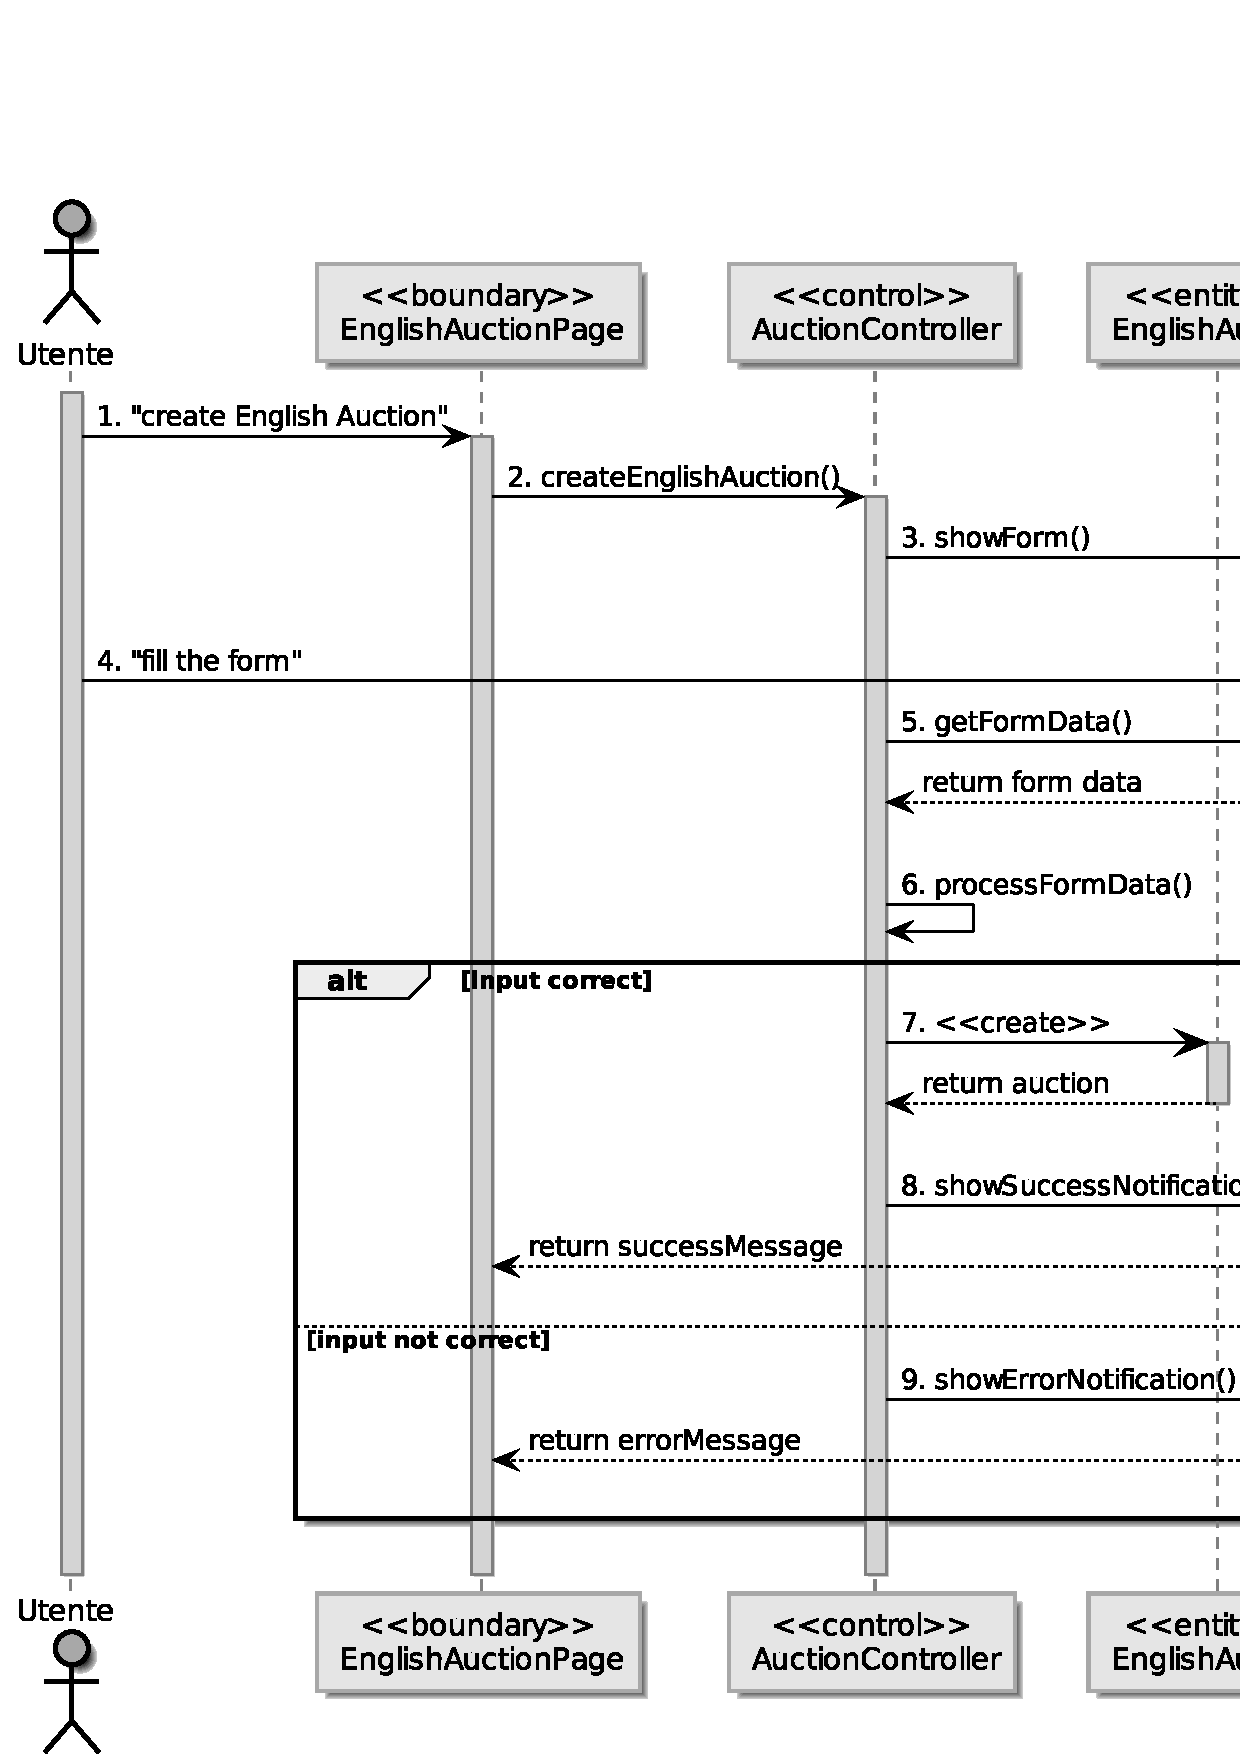
\includegraphics[width=\textwidth]{assets/sequence/creazione_asta_inglese.pdf}
\newpage

\subsection{Piazzare un'offerta su un'asta al ribasso}
Questo Sequence descrive il processo di creazione di un'offerta per un'asta al ribasso.\\
L'attore principale è l'utente acquirente che inizia il processo di creazione dell'offerta inserendo i dati all'interno del form e cliccando il pulsante di conferma.\\
Il sistema, dopo aver elaborato i dati, restituisce un messaggio all'utente.\bskip
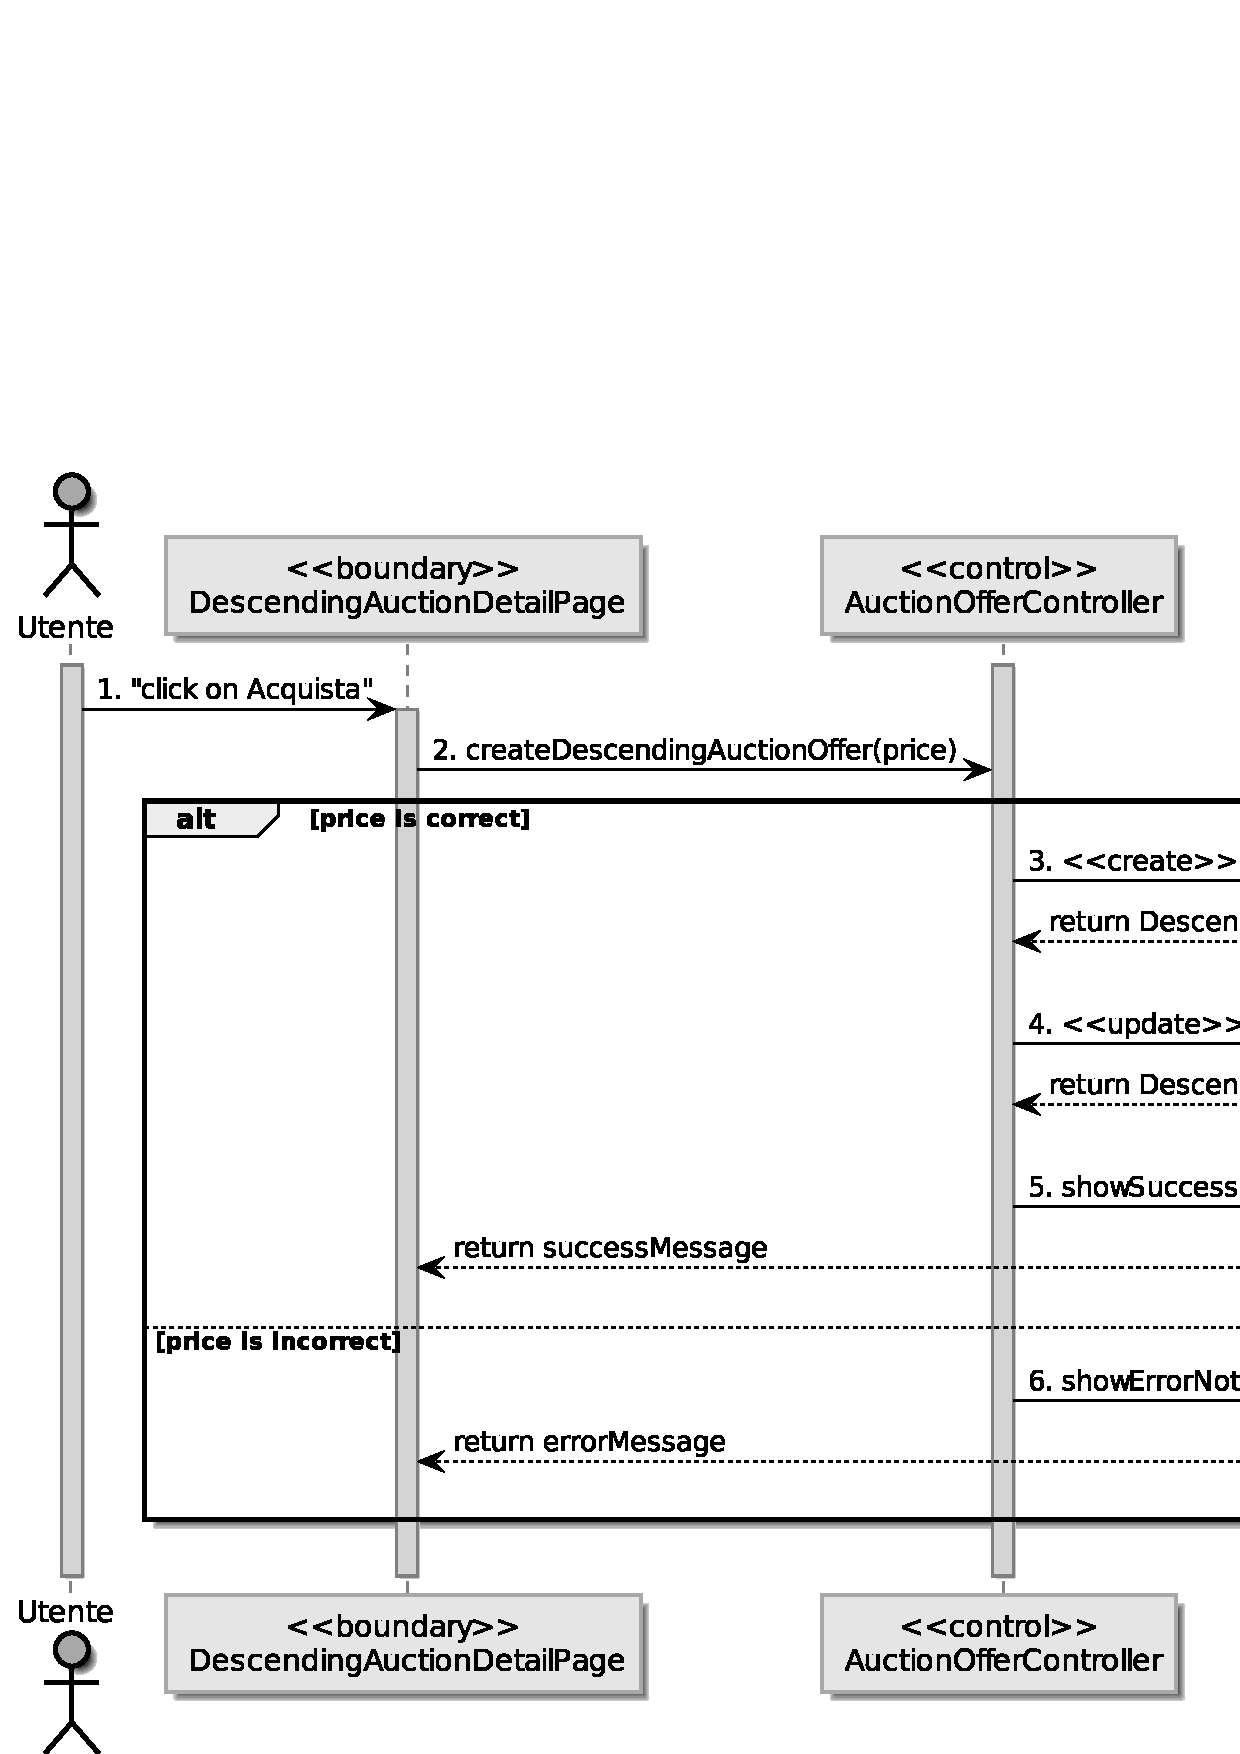
\includegraphics[width=\textwidth]{assets/sequence/piazzare_offerta_a_ribasso.pdf}
\newpage

\section{Progettazione degli Event-Based Statecharts}
Gli statecharts (o statechart diagrams) sono un tipo di diagramma utilizzato
per rappresentare il comportamento dinamico di un sistema attraverso
i suoi stati e le transizioni tra di essi.
\subsection{Creazione asta silenziosa}
Il seguente statechart descrive il comportamento del sistema durante la creazione di un'asta silenziosa.\\
Per prima cosa, l'utente si trova all'interno della schermata di selezione della tipologia d'asta da creare.
Dopo aver selezionato la tipologia d'asta corretta, il sistema passa alla pagina di creazione dell'asta, la quale contiene il form in cui inserire tutte le informazioni necessarie. Una volta che l'utente ha selezionato e inserito tutte le informazioni correttamente, l'asta viene creata e il sistema si aggiorna.\bskip
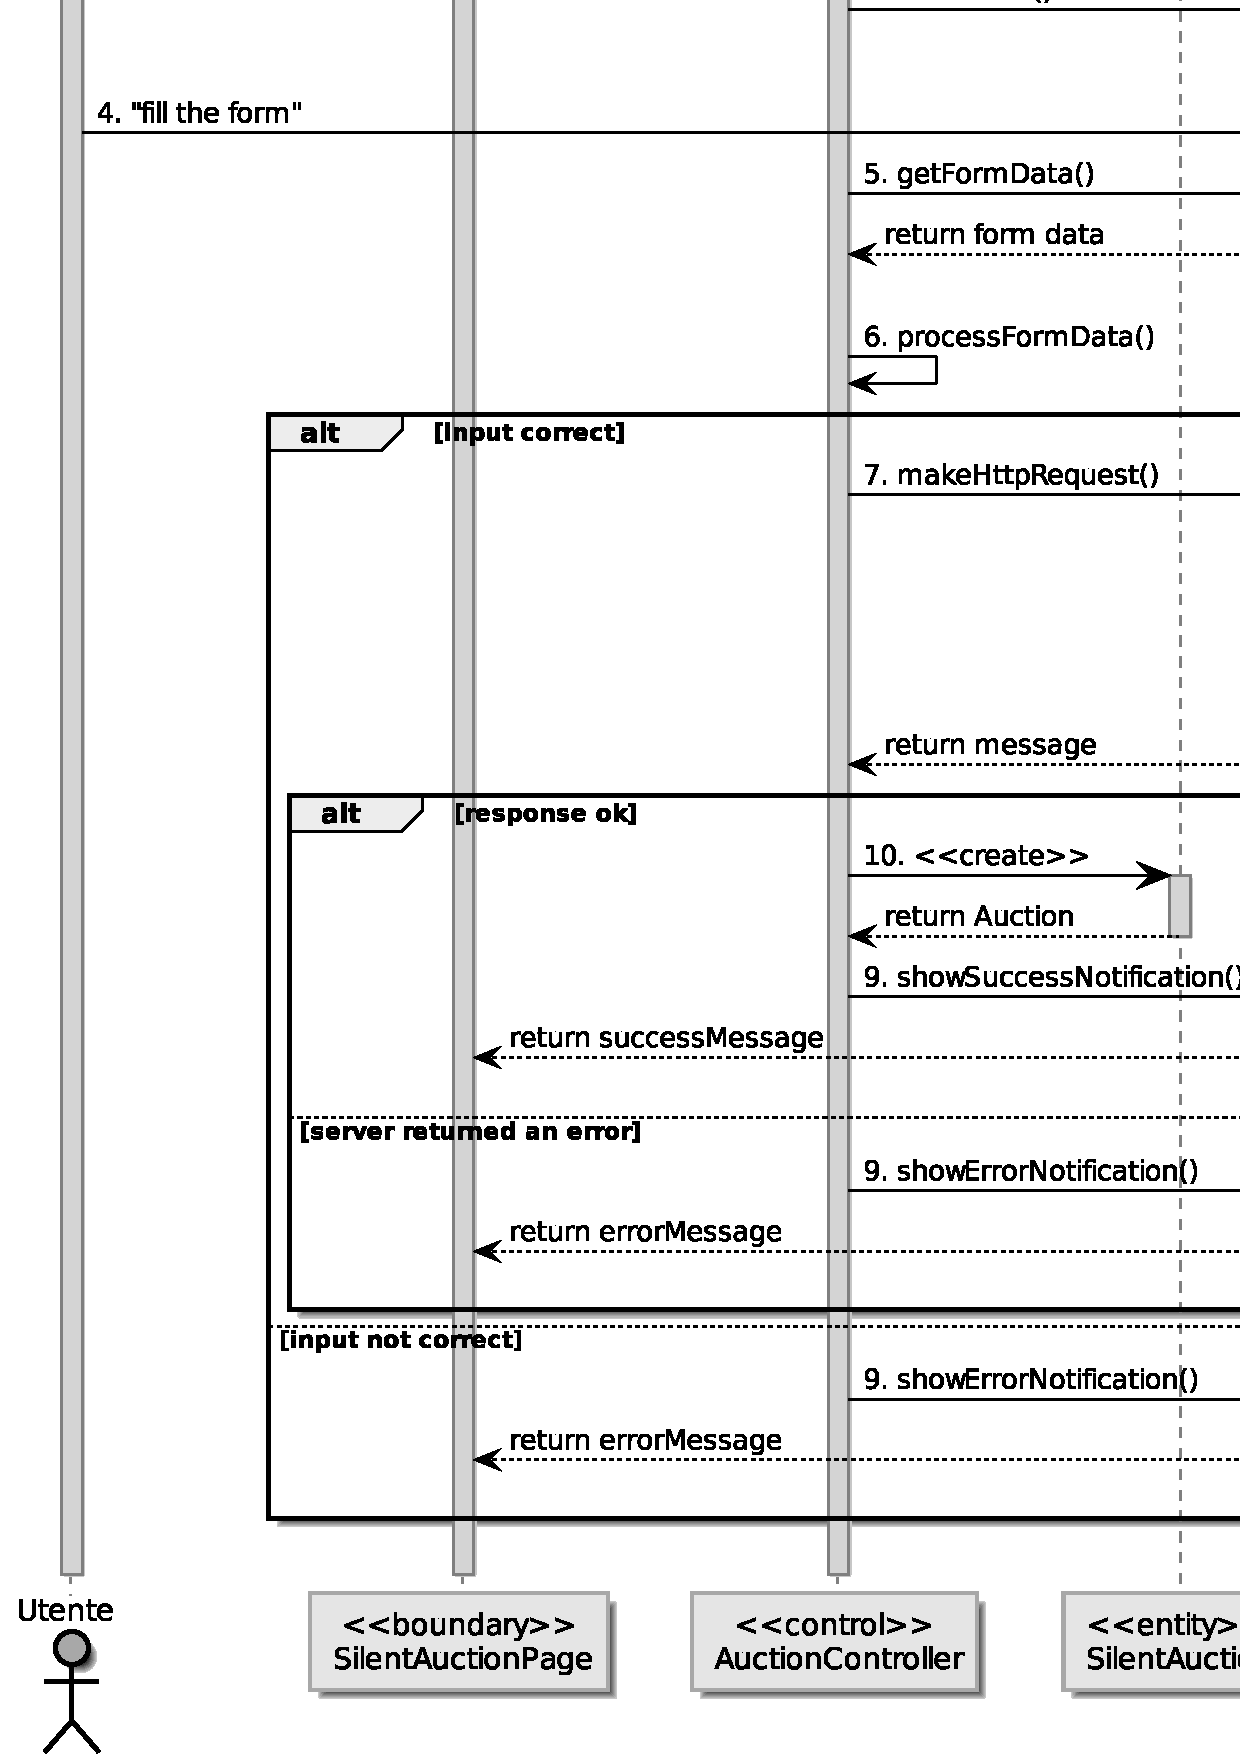
\includegraphics[width=\textwidth]{assets/state_charts/creazione_asta_silenziosa.pdf}
\newpage

\subsection{Offerta asta silenziosa}
Questo statechart descrive il comportamento del sistema durante la creazione di un'offerta per il tipo d'asta silenziosa.
Per prima cosa, l'utente seleziona l'asta cui desidera piazzare un'offerta.\\
Dopo aver effettuato la selezione il sistema passa alla schermata di dettaglio dell'asta, in cui è possibile inserire un'offerta.
Se l'offerta è corretta, il sistema si aggiorna correttamente.
\begin{center}
	\includegraphics[width=0.75\textwidth]{assets/state_charts/offerta_asta_silenziosa.pdf}
\end{center}
\newpage

\subsection{Aggiungi link social}
Questo statechart descrive il comportamento del sistema durante l'aggiunta di un link social. Nello specico, il sistema si trova in uno stato iniziale in cui è possibile visualizzare il profilo utente.
Dopodiche, il sistema passa nello stato di aggiornamento del profilo, in cui è possibile aggiungere un nuovo link social.
Dopo che il link è stato aggiunto, l'utente salva le modifiche e il sistema passa nello stato di profilo aggiornato.
\begin{center}
	\includegraphics[width=.75\textwidth]{assets/state_charts/aggiungi_link_social.pdf}
\end{center}
\newpage

\subsection{Visualizzare aste create}
Questo statechart descrive il comportamento del sistema quando l'utente vuole visualizzare lo storico delle aste create.
In particolare, il sistema può trovarsi in due sottostati diversi: schermata dello storico delle aste create, e la schermata dello storico delle aste acquistate.
Il sistema si ricorda dell'ultima schermata in cui si trovava precedentemente, che è di default la schermata delle aste create.
Da ognuna di queste due schermate è possibile passare all'altra.
\begin{center}
	\includegraphics[width=.75\textwidth]{assets/state_charts/visualizzare_aste_create.pdf}
\end{center}
\newpage